%------------------------------------------
%       $Id$
%
%       The GMT Documentation Project
%       Copyright (c) 2000-2012.
%       P. Wessel, W. H. F. Smith, R. Scharroo, and J. Luis
%------------------------------------------
%
\documentclass{report}
\newcommand{\GMTTITLE}{C/C++ Application Programming Interface}
\usepackage{ifpdf}
\usepackage{graphicx}
\usepackage{makeidx}
\usepackage{a4wide}
\usepackage{float}
\usepackage{GMT}
\usepackage{times}
\usepackage{color}
\usepackage{mathptmx}
\usepackage{verbatim}
\usepackage{tocbibind}
\usepackage{html}% Implies \usepackage{hyperref}

\input{GMT_version}

\newcommand{\GMTSITE}{gmt.soest.hawaii.edu}

\ifpdf
   % Here for creating PDF output with pdfLaTeX
   \pdfcompresslevel=9
   \DeclareGraphicsExtensions{.pdf}
   \hypersetup{%
      pdfauthor={Paul Wessel, Walter H. F. Smith},
      pdftitle={The Generic Mapping Tools Version \GMTDOCVERSION---\GMTTITLE},
      pdfsubject={GMT: Generic Mapping Tools},
      pdfkeywords={GMT, projections, mapping},
      pdfcreator={pdfLaTeX},
      bookmarksopen=true,
      bookmarksnumbered=true,
      hypertexnames=true,
      breaklinks=true,
      %pdfstartview={FitH},
      %linkbordercolor={1 1 0},
      %urlbordercolor={1 0 0},
   }%
   \newcommand{\GMT}{\textit{GMT}}
   \newcommand{\gmt}{\href{http://\GMTSITE}{\textbf{GMT}}}
   \newcommand{\GMTprogi}[1]{\htmladdnormallink{\textsfbf{#1}}{../html/#1.html}}
\else
   % Here for creating PS or HTML output with LaTeX
   \DeclareGraphicsExtensions{.eps}
   \newcommand{\GMT}{\htmladdnormallink{\includegraphics{fig/GMT_glyph10.eps}}{http://\GMTSITE}}
   \newcommand{\gmt}{\htmladdnormallink{GMT}{http://\GMTSITE}}
   \newcommand{\GMTprogi}[1]{\htmladdnormallink{\textsfbf{#1}}{../#1.html}}
\fi

\pagecolor{white}

% GMTfig will insert an eps file, add a label, and set a caption
\newcommand{\GMTfig}[3][tbp]{\begin{figure}[#1]\centering\includegraphics{scripts/#2}\caption{#3}\label{fig:#2}\end{figure}}
% Same for examples (scales by 50% by default)
\newcommand{\GMTexample}[3][scale=0.5]{\begin{figure}[hbtp]\centering\includegraphics[#1]{scripts/example_#2}\caption{#3}\label{fig:GMT_example_#2}\end{figure}}
\newcommand{\GMTanimation}[3][scale=0.5]{\begin{figure}[hbtp]\centering\includegraphics[#1]{scripts/anim_#2}\caption{#3}\label{fig:GMT_animation_#2}\end{figure}}

\newcommand{\PS}{\textit{PostScript}}
\newcommand{\UNIX}{\textit{UNIX}}
\newcommand{\id}[1]{#1\index{#1}}

\newcommand{\textsfbf}[1]{{\sffamily\bfseries #1\/}}
\newcommand{\textslbf}[1]{{\slshape\bfseries #1\/}}

\newcommand{\GMTprog}[1]{\GMTprogi{#1}\index{#1@\textsfbf{#1}}}

\newcommand{\script}[1]{%
   \begingroup
   \scriptsize\vspace{0.25\baselineskip}\noindent\hrulefill\vspace{-0.75\baselineskip}%
   \verbatiminput{scripts/#1.tex}%
   \vspace{-1.25\baselineskip}\noindent\hrulefill\vspace{0.25\baselineskip}%
   \endgroup
}

\newcommand{\GMTfunc}[1]{\texttt{#1}}
\newcommand{\filename}[1]{\underline{#1}}

\setcounter{topnumber}{2}
\renewcommand{\topfraction}{.8}
\setcounter{bottomnumber}{1}
\renewcommand{\bottomfraction}{.7}
\setcounter{totalnumber}{3}
\renewcommand{\textfraction}{.2}
\renewcommand{\floatpagefraction}{.7}

\sloppy

\newcommand{\DS}{$^{\circ}$}
\newcommand{\PM}{$\pm$}
\newcommand{\progname}[1]{\textslbf{#1}\index{#1@\textslbf{#1}}}
\newcommand{\Opt}[1]{\textbf{--#1}}

% Now overrule a few things for running LaTeX2HTML.
% Note that we need \gdef because they are inside an environment and would otherwise be local to
% that.
\begin{htmlonly}
   \gdef\GMT{\htmladdnormallink{\textbf{GMT}}{http://\GMTSITE}}
   \gdef\gmt{\GMT}
   \gdef\script#1{\htmlrule\verbatiminput{scripts/#1.tex}\htmlrule}
   \gdef\DS{�}
   \gdef\Opt#1{\textbf{-#1}}
   \gdef\PM{�}
   \gdef\progname#1{\textit{#1}\index{#1@\textit{#1}}}
\end{htmlonly}

% Restrict the indentation of lists
\setlength\leftmargin\parindent
\setlength\leftmargini\parindent
\setlength\leftmarginii\parindent
\setlength\leftmarginiii\parindent
\setlength\leftmarginiv\parindent
\setlength\leftmarginv\parindent
\setlength\leftmarginvi\parindent

\makeindex

%--------------------------------------------------------------------------
\begin{document}

\pagenumbering{roman}
%------------------------------------------
%       $Id: GMT_Cover.tex,v 1.28 2011-04-18 19:30:27 remko Exp $
%
%       The GMT Documentation Project
%	Copyright (c) 2000-2011.
%	P. Wessel, W. H. F. Smith, R. Scharroo, and J. Luis
%------------------------------------------
%

\thispagestyle{empty}

\begin{center}
\Huge
\textbf{The Generic Mapping Tools}\par 
\vspace{0.5\baselineskip}
\textbf{\GMTTITLE}\par 

\large
\vspace{0.5\baselineskip}
\textbf{Version \GMTDOCVERSION, \GMTDOCDATE}\par 
\vspace{0.25\baselineskip}

\vspace{2.0\baselineskip}

\huge
\textbf{P\aa l (Paul) Wessel}\par 
\vspace{0.5\baselineskip}

\Large
\textbf{SOEST, University of Hawai'i at M\={a}noa}\par 
\vspace{0.5\baselineskip}

\huge
\textbf{Walter H. F. Smith}\par 
\vspace{0.5\baselineskip}

\Large
\textbf{Laboratory for Satellite Altimetry, NOAA/NESDIS}\par 
\vspace{0.5\baselineskip}

\huge
\textbf{Remko Scharroo}\par 
\vspace{0.5\baselineskip}

\Large
\textbf{Altimetrics LLC, Cornish, New Hampshire}\par 
\vspace{0.5\baselineskip}

\huge
\textbf{Joaquim Luis}\par 
\vspace{0.5\baselineskip}

\Large
\textbf{Universidade do Algarve, Faro, Portugal}\par 
\vspace{0.5\baselineskip}



\includegraphics{GMT_coverlogo}
\end{center}

\addcontentsline{toc}{chapter}{Front page}
\clearpage

\thispagestyle{headings}

\tableofcontents 
\thispagestyle{headings}

\chapter{Introduction} 
\index{Introduction}
\pagenumbering{arabic}
\thispagestyle{headings}
\index{Purpose of the GMT API}
\index{GMT API!Purpose}

\section{Preamble}
\index{Preamble}

\begin{figure}[h]
	\centering
	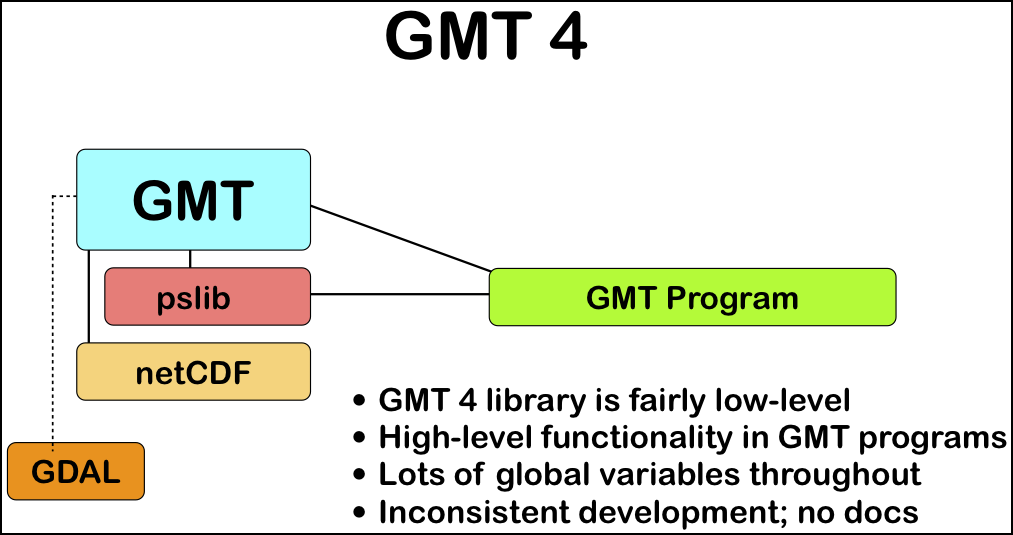
\includegraphics[width=10cm,bb=0 0 485 255]{GMT4_mode.png}
	\caption{GMT 4 programs contain all the high-level functionality.}
\end{figure}
Prior to version 5, the bulk of \GMT\ functionality was coded directly
in the standard \GMT\ C program modules (e.g., \filename{surface.c}, \filename{psxy.c}, \filename{grdimage.c}).
The \GMT\ library only offered access to lower-level functions from which those
high-level \GMT\ programs were built.  The standard \GMT\ programs have been very successful,
with tens of thousands of users world-wide.  However, the design of the main programs
prevented developers from leveraging \GMT\ functionality from within other
programming environments since access to \GMT\ tools could only be achieved
via system calls.  Consequently, all data i/o had to be done via temporary files.
The design also prevented the \GMT\ developers themselves from taking advantage of these
modules directly.  For instance, the tool \GMTprog{pslegend} needed to make extensive use of system calls
to \GMTprog{psxy} and \GMTprog{pstext} in order to plot the lines, symbols and text
that make up a map legend.

\begin{figure}[h]
	\centering
	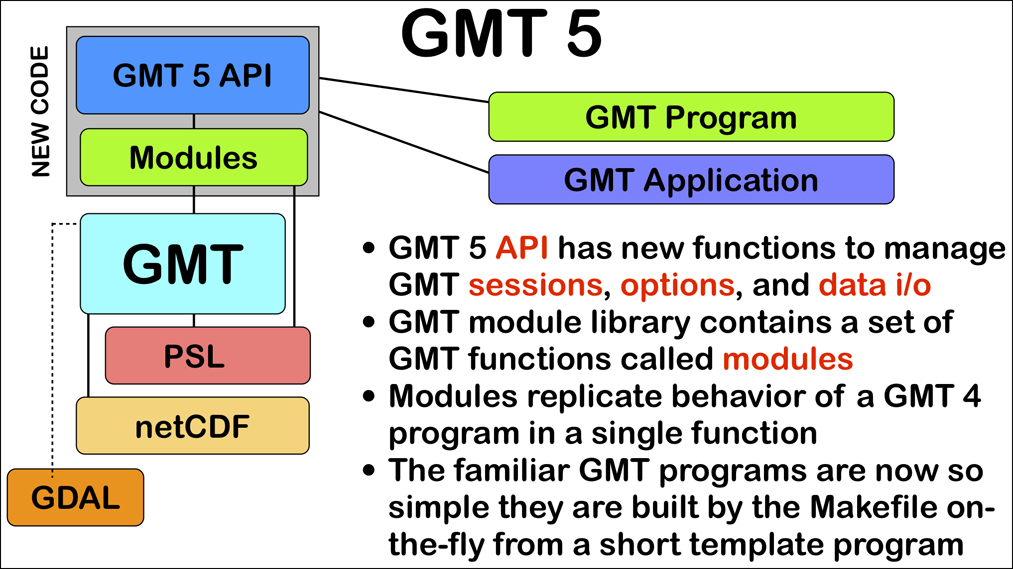
\includegraphics[width=10cm,bb=0 0 485 255]{GMT5_mode.png}
	\caption{GMT 4 programs contain all the high-level functionality.}
\end{figure}
Starting with \GMT\ version 5, all standard \GMT\ programs are split into short driver
program (the ``new'' \GMT\  programs) and a function ``module''.  The drivers simply call the corresponding \GMT\ modules;
it is these modules that do most of the work.  These new functions have been placed
in a new \GMT\ high-level API library and can be called from a variety of environments
(C/C++, Fortran, Python, Matlab, Visual Basic, etc.)\footnote{Currently, only C/C++ and Matlab are being tested.}.
For example, the main program
\filename{blockmean.c} has been reconfigured as a high-level function \GMTfunc{GMT\_blockmean()},
which does the actual spatial averaging and passes the result back to the calling program.
The previous behavior of \filename{blockmean.c} is replicated by a short driver program
that simply collects user arguments and then calls \GMTfunc{GMT\_blockmean()}.  Indeed, the driver
programs for all the standard \GMT\ programs are so short and simple that the makefile generates them
on-the-fly when it compiles and links them with the \GMT\ library into executables.
Thus, \filename{blockmean.c} and others do no longer exist.

In order for this interface to be as flexible as possible we have generalized the notion of input
and output. Now, data that already reside in an application's memory may serve as
input to a \GMT\ function.  Other sources of input may be file pointers
and file descriptors (as well as the already-supported mechanism for passing file names).
For standard data table i/o, the \GMT\ API takes care of the task of assembling any combination
of files, pointers, and memory locations into a single virtual data set from which the \GMT\
function may read (a) all records at once into memory, or (b) read one record at a time.
Likewise, \GMT\ functions may write their output to a virtual destination, which
might be a memory location in the user's application, a file pointer or descriptor, or
an output file.  The \GMT\ functions are unaware of these details and simply
read from a ``source'' and write to a ``destination''.

Here, we document the new functions in the \GMT\ API library for application developers
who wish to call these functions from their own custom programs.  At this point,
only the new high-level \GMT\ API is fully documented and intended for public use.
The structure and documentation of the under-lying lower-level \GMT\ library is not finalized
Developers using these functions may risk disruption to their programs due to changes we may
make in the library in support of the \GMT\ API.

\section{Definitions}

For the purpose of this documentation a few definitions are needed:

\begin{enumerate}
\item ``Standard \GMT\ program'' refers to one of the traditional stand-alone command-line
executables known to all \GMT\ users, e.g., \GMTprog{blockmean}, \GMTprog{psxy},
\GMTprog{grdimage}, etc.  Prior to version 5, these were the only \GMT\ executables available.
\item ``\GMT\ module'' refers to the function in the \GMT\ API
library that is responsible for all the action taken by the corresponding \GMT\ program.  All
such modules are given the same name as the corresponding program but carry the
prefix \texttt{GMT\_}, e.g., \texttt{GMT\_blockmean}.
\item ``\GMT\ application'' refers to a new application written by developers
and may call one or more \GMT\ functions to create a new \GMT-compatible executable.
\item In the API description that follows we will use the type \texttt{long} to mean
a 4-byte (for 32-bit systems) or 8-byte (for 64-bit systems) integer.  Since different
operating systems have their own way of defining 8-byte integers it is recommended that
developers use the type \texttt{GMT\_LONG} for this purpose; it is guaranteed to yield
the correct type that the \GMT\ functions expect.
\end{enumerate}
In version 5, the standard \GMT\ programs are themselves specific but overly simple examples
of \GMT\ applications that only call the single \GMT\ function they are associated with.
However, some exceptions such as \GMTprog{pslegend} and \GMTprog{gmtconvert} call several modules.

\section{Recognized resources}
\index{Recognized resources}
\index{Resources!Recognized by GMT}

The \GMT\ API knows how to read and write five types of data common to \GMT\ operations:
CPT palette tables, data tables (ASCII or binary), text tables, \GMT\ grids and images (reading only).
In addition, we have two data types to facilitate the passing of simple user arrays (one or more data columns
of any data type, e.g., double, char) and 2-D user matrices (of any data type and column/row organization).
There are many attributes for each of these two entities and therefore we use a top-level structure for each
to keep them all in one container.  These containers are given or returned by the \GMT\ API
functions using pointers (\texttt{void *}).  Below we discuss these containers in some detail; we
will later present how they are used when importing or exporting them to or from files,
memory locations, or streams.  The first five are the standard \GMT\ objects, while the latter two are the
special user data containers.

\subsection{CPT palette tables}
\index{CPT palette tables}
\index{Resources!CPT palette tables}

The color palette table files, or just CPT tables, contain colors and patterns used for plotting
data such as surfaces (i.e., \GMT\ grids) or symbols, lines and polygons (i.e., \GMT\ tables).
\GMT\ programs will generally read in a CPT
palette table, make it the current palette, do the plotting, and destroy the table when done.
The information is referred to via a pointer to \texttt{struct GMT\_PALETTE}.  Thus, the
arguments to \GMT\ API functions that handle palettes expect this type of variable.

\subsection{Data tables}
\index{Data tables}
\index{Resources!Data tables}

Much data processed in \GMT\ come in the form of ASCII or binary data tables.  These may
have any number of header records (ASCII only) and perhaps segment headers.  \GMT\ programs will
read one or many such tables when importing data.  However, to avoid memory duplication some programs may prefer to read
records one at the time.  The \GMT\ API has functions that let you read record-by-record
by presenting a virtual data set that combines all the data tables specified as input.
This simplifies record processing considerably.  A \texttt{struct GMT\_DATASET} may contain
any number of tables, each with any number of segments, and each segment with any number of records.   Thus, the
arguments to \GMT\ API functions that handle such data sets expect this type of variable.  All segments
are expected to have the same number of columns.

\subsection{Text tables}
\index{Text tables}
\index{Resources!Text tables}

Some data needed by \GMT\ are simply free-form ASCII text tables.  These are handled
similarly to data tables.  E.g., they may have any number of header records and even segment headers,
and \GMT\ programs can read one or more tables or get text records one at the time.
A \texttt{struct GMT\_TEXTSET} may contain
any number of tables, each with any number of segments, and each segment with any number of records.   Thus, the
arguments to \GMT\ API functions that handle such data sets expect this type of variable.

\subsection{GMT grids}
\index{GMT grids}
\index{Resources!GMT grids}

\GMT\ grids are used to represent equidistant and organized 2-D surfaces.  These can be
plotted as contour maps, color images, or as perspective surfaces.  Because the native
\GMT\ grid is simply a 1-D float array with all the metadata kept in a separate header, we
pass this information via a \texttt{struct GMT\_GRID}, which is a container that holds both items.
Thus, the arguments to \GMT\ API functions that handle such \GMT\ grids expect this type
of variable.

\subsection{GMT images}
\index{GMT images}
\index{Resources!GMT images}

\GMT\ images are used to represent bit-mapped images obtained via the GDAL bridge.  These can be
reprojected internally, such as when used in grdimage.  Since images and grids share the concept
of a header, we use the same header structure for grids as for images; however, some additional
metadata attributes are also needed.  Finally, the image itself may be of any data type.
Both image and header information are passed via a \texttt{struct GMT\_IMAGE}, which is a container that holds both items.
Thus, the arguments to \GMT\ API functions that handle such \GMT\ images expect this type
of variable.  Unlike the other objects, images can only be read and not written.

\subsection{User data columns}
\index{User data columns}
\index{Resources!User data columns}

\begin{table}[h]
\small
\centering
\begin{tabular}{ll} \hline
\multicolumn{2}{l}{\texttt{union GMT\_UNIVECTOR \{}} \\ 
\texttt{	unsigned char *uc1;}	&       /* \emph{Pointer for unsigned char array} */ \\
\texttt{	char *sc1;}		&       /* \emph{Pointer for signed char array} */ \\
\texttt{	unsigned short *ui2;}	&       /* \emph{Pointer for unsigned short array} */ \\
\texttt{	short *si2;}		&       /* \emph{Pointer for signed short array} */ \\
\texttt{	unsigned int *ui4;}	&       /* \emph{Pointer for unsigned int array} */ \\
\texttt{	int *si4;}		&       /* \emph{Pointer for signed int array} */ \\
\texttt{	unsigned long *ui8;}	&       /* \emph{Pointer for unsigned long array} */ \\
\texttt{	long *si8;}		&       /* \emph{Pointer for signed long array} */ \\
\texttt{	float *f4;}		&       /* \emph{Pointer for float array} */ \\
\texttt{	double *f8;}		&       /* \emph{Pointer for double array} */ \\
\texttt{\};}	&        \\  \hline
\end{tabular}
\caption{Definition of the GMT\_UNIVECTOR union that hold a pointer to any array type.}
\label{tbl:univector}
\index{Vectors!Structure}
\end{table}

\begin{table}[h]
\small
\centering
\begin{tabular}{ll} \hline
\multicolumn{2}{l}{\texttt{struct GMT\_VECTOR \{}} \\ 
\texttt{	long id;}		&       /* \emph{An identification number} */ \\
\texttt{	long n\_rows;}		&       /* \emph{Number of rows in each vector} */ \\
\texttt{	long n\_columns;}	&       /* \emph{Number of vectors}  */\\
\texttt{	long alloc\_mode;}	&       /* \emph{Determines if we may free the vectors or not}  */\\
\texttt{	long *type;}		&       /* \emph{Array with data type for each vector}  */\\
\texttt{	union GMT\_UNIVECTOR *data;}	&       /* \emph{Array with unions for each column}  */\\
\texttt{\};}	&        \\  \hline
\end{tabular}
\caption{Definition of the GMT\_VECTOR structure used to pass user data columns.}
\label{tbl:vector}
\index{Vectors!Structure}
\end{table}
\noindent
Programs that may wish to call \GMT\ modules may have input data in their own particular
structures.  For instance, the user's program may have three column arrays of type float
and wishes to use these as the input source to the \texttt{GMT\_surface} module, which normally
expects a \texttt{struct GMT\_DATASET} via file or reference.  Simply create a \texttt{struct GMT\_VECTOR}
(see section~\ref{sec:create}) and assign the union array pointers  (see Table~\ref{tbl:univector}) to your data columns and provide
the required information on length and data types (see Table~\ref{tbl:vector}).
By letting the \GMT\ module know you are passing a data set via a \texttt{struct GMT\_VECTOR} it will know how to
read the data properly.

\subsection{User data matrices}
\index{User data matrices}
\index{Resources!User data matrices}

\begin{table}[h]
\small
\centering
\begin{tabular}{ll} \hline
\multicolumn{2}{l}{\texttt{struct GMT\_MATRIX \{}} \\ 
\texttt{	long id;}		&       /* \emph{An identification number} */ \\
\texttt{	long n\_rows;}		&       /* \emph{Number of rows in the matrix} */ \\
\texttt{	long n\_columns;}	&       /* \emph{Number of columns in the matrix}  */\\
\texttt{	long n\_layers;}	&       /* \emph{Number of layers in a 3-D matrix}  */\\
\texttt{	long registration;}	&       /* \emph{0 for gridline and 1 for pixel registration}  */\\
\texttt{	long shape;}		&       /* \emph{0 = C (rows) and 1 = Fortran (cols)}  */\\
\texttt{	long dim;}		&       /* \emph{Length of dimension for row (C) or column (Fortran)}  */\\
\texttt{	long alloc\_mode;}	&       /* \emph{Determines if we may free the vectors or not}  */\\
\texttt{	long type;}		&       /* \emph{The matrix data type}  */\\
\texttt{	double limit[6];}	&       /* \emph{The min and max limits on x-, y-, and z-ranges}  */\\
\texttt{	union GMT\_UNIVECTOR data;}	&       /* \emph{Union with pointers a data matrix of any type}  */\\
\texttt{\};}	&        \\  \hline
\end{tabular}
\caption{Definition of the GMT\_MATRIX structure used to pass a user data matrix.}
\label{tbl:matrix}
\index{Matrix!Structure}
\end{table}
\noindent
Likewise, a programs may have an integer 2-D matrix in memory 
and wish to use that as the input grid to the \texttt{GMT\_grdfilter} module, which normally
expects a \texttt{struct GMT\_GRID} via file or reference.  As for user vectors, we create a
\texttt{struct GMT\_MATRIX} (see section~\ref{sec:create}), assign the appropriate union pointer to your data
matrix and provide information on dimensions and data type (see Table~\ref{tbl:matrix}).
Letting the \GMT\ module know you are passing a grid via a
\texttt{struct GMT\_MATRIX} it will know how to read the matrix properly.

\chapter{Overview of the GMT C Application Program Interface}
\index{C interface}
\index{Interface!C}

Users who wish to create their own \GMT\ applications based on the API
must make sure their program goes through the steps below; details
for each step will be revealed in the sections to follow.  We have kept the
API simple: In addition to the \GMT\ modules, there are only 17 public functions to become familiar with.
All functions sets the variable \texttt{API->error} to the appropriate error code (when things go wrong);
otherwise it is set to GMT\_OK (0).
The layout here assumes you wish to use data in memory as input sources; if the data are simply
command-line files then things simplify considerably.

\begin{enumerate}
\item Initialize a new \GMT\ session by calling \texttt{GMT\_Create\_Session}, which
allocates a \GMT\ API control structure and returns a pointer to it.  This pointer must be used
as first argument to all subsequent \GMT\ API function calls within the same session.
\item For each intended call to a \GMT\ function, several steps are involved:
\begin{enumerate}
\item Register the input sources and register the output destination
using \texttt{GMT\_Register\_IO}, unless you know you are working with a single file
or standard input/output.
The resources will typically be files, memory locations, already-opened file handles,
and even process streams.
\item Each resource registration will generate a unique ID number.  For memory resources, these numbers are
then converted to unique filenames of the form ``@GMTAPI@-\#\#\#\#\#\#'' that are used with \GMT\ modules.  When
\GMT\ i/o library functions encounter such filenames they extract the ID and make a connection
to the resource registered under that ID.  Any number of table data or text sources
will be combined into a single virtual source for \GMT\ functions to operate on.
In contrast, CPT, Grid, and image resources are operated on individually.
\item Enable data import once all registrations are complete.
\item Read into memory all data that will be passed to \GMT\ modules via pointers.  You may choose
	to read everything into memory at once or process the data record-by-record (tables only).
\item Prepare the program options required and call the \GMT\ module you wish to use.
\item Process the results that were returned to memory via pointers rather than written to files.
\item Explicitly destroy the resources allocated by \GMT\ modules to hold the results, or let the
garbage collector do this automatically at the end of the module and at the end of the session.
\end{enumerate}
\item Repeat steps a--f as many times as your application requires.  All API functions
return a status code which is GMTAPI\_OK (0) if all is well.  For non-zero return values, use
\texttt{GMT\_Report\_Error} to generate an error message.
\item We terminate the GMT session by calling \texttt{GMT\_Destroy\_Session}.
\end{enumerate}

Advanced programs may be calling more than one \GMT\ session and thus run several
sessions, perhaps  concurrently as different threads on multi-core machines.
We will now discuss these steps in more detail.

\section{Initialize a new GMT\ session}
\index{Initialize a new GMT session}
\index{GMT session!Initialize}

Most applications will need to initialize only a single \GMT\ session.  This is true of all
the standard \GMT\ programs since they only call one \GMT\ module and then exit.  Most
user-developed \GMT\ applications are likely to only initialize one session even though
they may call many \GMT\ modules.  However, the \GMT\ API supports any number of
simultaneous sessions should the programmer wish to take advantage of it.  This
might be useful when you have access to several CPUs and want to spread the computing load\footnote{However,
there is no thread-support yet.}.
In the following discussion we will simplify our treatment to the use
of a single session only.

The \texttt{GMT\_Create\_Session} is used to initiate the new session.  The full
function prototype is
\index{GMT\_Create\_Session}

\begin{verbatim}
struct GMTAPI_CTRL * GMT_Create_Session (char *tag, long mode)
\end{verbatim}
and you will typically call it thus:
\begin{verbatim}
GMT_LONG mode = GMTAPI_GMT;
struct GMTAPI_CTRL *API = NULL;
API = GMT_Create_Session ("Session name", mode);
\end{verbatim}
where \texttt{API} is a pointer to the allocated \GMT\ API control structure.  You will need to
pass this pointer to \emph{all} subsequent \GMT\ API functions.  The key task of this initialization
is to set up the \GMT\ machinery and its internal variables used for map projections, plotting,
etc.  The initialization also allocates space for internal structures used to register resources.
If you expect to call modules that also require the PSL library, then set \texttt{mode} to
GMTAPI\_GMTPSL (1); else simply pass GMTAPI\_GMT (0).  Should something go wrong then \texttt{API}
will be returned as \texttt{NULL}.

\section{Register input or output resources}
\index{Register input or output resources}
\index{Resources!Register}
\index{Resources!Input}
\index{Resources!Output}
\index{Sources!Register Input}
\index{Sources!Register Output}

When using the standard \GMT\ programs, you specify input files on
the command line or via special program options (e.g., \Opt{I}\emph{intensity.nc}). The output of
the programs are either written to standard output (which you redirect to files or pipe to other programs)
or to files specified by specific program options (e.g., \Opt{G}\emph{output.nc}).  However, the
\GMT\ API allows you to also specify input (and output) to come from (or go to) open file handles
or program memory locations.  We will examine this more closely below.  Registering a
resource is a required step before attempting to import or export data other that via file options
and standard input/output.

\subsection{Resource registration}
The basic registration machinery involves a direct or indirect call to
\index{GMT\_Register\_IO}

\begin{verbatim}
long GMT_Register_IO (struct GMTAPI_CTRL *API, long family, long method, \
   long geometry, long direction, void *ptr, double wesn[])
\end{verbatim}
where \texttt{family} specifies what kind of resource is to be registered
(see Table \ref{tbl:family} for list of all families), \texttt{method} specifies
how we expect to access this resource (see Table \ref{tbl:methods} for recognized methods,
as well as modifiers you can add; these are listed in Table \ref{tbl:via}),
\texttt{geometry} specifies
the geometry of the data (see Table \ref{tbl:geometry} for recognized geometries),
\texttt{ptr} is the address of the pointer to the named input resource.  If \texttt{direction}
is GMT\_OUT and the \texttt{method} is not related to a file (filename, stream, or handle),
then \texttt{ptr} must be NULL.  After the \GMT\ module has written the data you can use
\texttt{GMT\_Retrieve\_Data} to assign a pointer to the memory location where the output container was allocated.
For grid (and image) resources you may request to obtain a subset via the \texttt{wesn}
array (see Table~\ref{tbl:wesn} for information); otherwise, pass NULL to obtain the entire grid (or image).
The \texttt{direction} indicates input or output and is either GMT\_IN (0) or GMT\_OUT (1).
Finally, the function returns a unique resource ID, or GMTAPI\_NOTSET (-1) if there was an
error (with error code returned via \texttt{API->error}).

\subsection{Object ID encoding}
If registered resources are to be given as program input or output arguments you will need to pass them via
a text string that represents a special file name.  The proper filename formatting is guaranteed by using the
function
\index{GMT\_Encode\_ID}

\begin{verbatim}
long GMT_Encode_ID (struct GMTAPI_CTRL *API, char *filename, long ID)
\end{verbatim}
which accepts the unique \texttt{ID} and writes the \texttt{filename} that
you can use as argument to a program option.  \texttt{filename} must have enough space to hold 16 bytes.
The function returns TRUE (1) if there is an error (which is passed back with \texttt{API->error}),
otherwise it returns FALSE (0).


\begin{table}[h]
\small
\centering
\begin{tabular}{|l|l|} \hline
\multicolumn{1}{|c|}{\emph{family}} & \multicolumn{1}{c|}{\emph{source points to}} \\ \hline
GMT\_IS\_DATASET		&       A [multi-segment] table file \\ \hline
GMT\_IS\_TEXTSET		&       A [multi-segment] text file \\ \hline
GMT\_IS\_GMTGRID		&       A \GMT\ grid file \\ \hline
GMT\_IS\_CPT			&       A CPT file \\ \hline
\end{tabular}
\caption{Integer constants defined for use when specifying input or output data families.}
\label{tbl:family}
\index{Resources!Parameters!Floating point}
\end{table}


\begin{table}[h]
\small
\centering
\begin{tabular}{|l|l|} \hline
\multicolumn{1}{|c|}{\emph{method}} & \multicolumn{1}{c|}{\emph{how to read/write data}} \\ \hline
GMT\_IS\_FILE		&       Pointer to name of a file \\ \hline
GMT\_IS\_STREAM		&       Pointer to open file (or process)  \\ \hline
GMT\_IS\_FDESC		&       Pointer to integer file descriptor \\ \hline
GMT\_IS\_COPY		&       Pointer to memory to \emph{copy} data from \\ \hline
GMT\_IS\_REF		&       Pointer to memory to \emph{reference} data from (realloc OK) \\ \hline
GMT\_IS\_READONLY	&       Pointer to memory to \emph{read} data from \\ \hline
\end{tabular}
\caption{Integer constants defined for use when specifying input or output methods.}
\label{tbl:methods}
\index{Resources!Methods}
\end{table}

\begin{table}[h]
\small
\centering
\begin{tabular}{|l|l|} \hline
\multicolumn{1}{|c|}{\emph{approach}} & \multicolumn{1}{c|}{\emph{how method is modified}} \\ \hline
GMT\_VIA\_VECTOR	&       The user's data columns are addressed via a GMT\_VECTOR structure \\ \hline
GMT\_VIA\_MATRIX	&       The user's grid is addressed via a GMT\_MATRIX structure \\ \hline
\end{tabular}
\caption{Integer constants defined for use when user data forms are involved.  These are to be added
to the \emph{method} used when registering the resource.}
\label{tbl:via}
\index{Resources!Conversions}
\end{table}

\begin{table}[h]
\small
\centering
\begin{tabular}{|l|l|} \hline
\multicolumn{1}{|c|}{\emph{geometry}} & \multicolumn{1}{c|}{\emph{description}} \\ \hline
GMT\_IS\_TEXT		&       Not a geographic item \\ \hline
GMT\_IS\_POINT		&       Multi-dimensional point data \\ \hline
GMT\_IS\_LINE		&       Geographic or Cartesian line segments \\ \hline
GMT\_IS\_POLYGON	&       Geographic or Cartesian closed polygons \\ \hline
GMT\_IS\_SURFACE	&       2-D gridded surface \\ \hline
\end{tabular}
\caption{Integer constants defined to register different geometries.}
\label{tbl:geometry}
\index{Resources!Geometries}
\end{table}

\begin{table}[h]
\small
\centering
\begin{tabular}{|c|l|l|} \hline
\multicolumn{2}{|c|}{\emph{Index}} & \multicolumn{1}{c|}{\emph{content}} \\ \hline
0 & XLO	&       x\_min (west) boundary of grid subset  \\ \hline
1 & XHI	&       x\_max (east) boundary of grid subset  \\ \hline
2 & YLO	&       y\_min (south) boundary of grid subset  \\ \hline
3 & YHI	&       y\_max (north) boundary of grid subset  \\ \hline
\end{tabular}
\caption{Domain boundaries (\texttt{wesn}) used when selecting subsets of grids.}
\label{tbl:wesn}
\index{Resources!Parameters!Domain}
\end{table}

\subsection{Resource initialization}
\index{Resources!Initialization}
\index{Initialization!Resources}
All \GMT\ programs dealing with (a) input or output files given on the command line or (b) defaulting to
the standard input or output streams if no files are given, must call the i/o initializer function
\texttt{GMT\_Init\_IO} once for each direction required (i.e., input and output).
For input it will determine how many input sources have already been registered.
If none have been registered then it will scan the program arguments for any filenames given on the command line, and register
these input resources.  Finally, if we still have found no input sources we will specify the standard input stream
as the single input source.  Likewise, for output: If no single destination has been registered we specify the standard output stream
as the output destination.  Only one output destination is allowed to be active when the module writes data.
The prototype for this function is
\index{GMT\_Init\_IO}

\begin{verbatim}
long GMT_Init_IO (struct GMTAPI_CTRL *API, long family, long geometry, \
    long direction, long mode, struct GMT_OPTION *head)
\end{verbatim}
where \texttt{family} specifies what kind of resource is to be registered,
\texttt{geometry} specifies the geometry of the data,
the \texttt{direction} is either \texttt{GMT\_IN} or \texttt{GMT\_OUT}, the
\texttt{mode} is a bit flag that determines what we do if no resources have been
registered. The choices are
\begin{description}
	\item [1] (or GMT\_REG\_FILES\_IF\_NONE) means ``add command line (option) files if none have been registered already''
	\item [2] (or GMT\_REG\_FILES\_ALWAYS) means ``always add any command line files''
	\item [4] (or GMT\_REG\_STD\_IF\_NONE) means ``add std* if no other input/output have been specified''
	\item [8] (or GMT\_REG\_STD\_ALWAYS) means ``always add std* even if resources have been registered''.
\end{description}
The standard behavior is 5 (or GMT\_REG\_DEFAULT).
Finally, \texttt{head} is the first element of the option structure list.

Many programs will register an export location to hold the results of a \GMT\ function (say,
a filtered grid), but then wish to use that location as an \emph{input} resource in the next
step.  This is accomplished by re-registering the same array
location as an import source, thereby changing the \emph{direction} of the data set.
The function returns TRUE (1) if there is an error (which is passed back with \texttt{API->error}),
otherwise it returns FALSE (0).

\subsection{Dimension parameters for user column vectors}
We refer to Table~\ref{tbl:vector}.  The \texttt{type} array must hold the
data type of each data column in the user's program.  All types other than GMTAPI\_DOUBLE will need
to be converted internally in \GMT\ to \texttt{double}, thus possibly increasing memory requirements.
If the type is GMTAPI\_DOUBLE then \GMT\ will be able to use the column directly by reference.  The \texttt{n\_columns}
and \texttt{n\_rows} parameters inform of the number of vectors and their common length.  These are known in
the case of input but may be unknowable in the case of output; if so you may pass 0 for these values
and set \texttt{alloc\_mode} to 1; this will make
sure \GMT\ will allocate the necessary memory at the location you specify.

\subsection{Dimension parameters for user 2-D table arrays}

We refer to Table~\ref{tbl:matrix}.  The \texttt{type} parameter specifies the
data type used for the array in the user's program.  All types other than GMTAPI\_FLOAT will need
to be converted internally in \GMT\ to \texttt{float}, thus possibly increasing memory requirements.
If the type is GMTAPI\_FLOAT then \GMT\ may be able to use the matrix directly by reference.  The \texttt{n\_rows}
and \texttt{n\_columns} parameters simply specify the dimensions of the matrix.  These are known in
the case of input but may be unknowable in the case
of output; if so you may pass 0 for these values and set \texttt{alloc\_mode} to 1; this will make
sure \GMT\ will allocate the necessary memory at the location you specify.  Fortran users
will instead have to specify a size large enough to hold the anticipated output data.
The \texttt{registration} and \texttt{limit} gives the grid registration and domain.
Finally, use the \texttt{dim} entry to indicate if the memory matrix has a dimension that
exceeds that of the leading row (or column) dimension. Note: For GMT\_IS\_TEXTSET
the user matrix is expected to be a 2-D character array with row length by \texttt{dim]}
but we only consider the first \texttt{n\_columns} characters.  For data grids you will
also need to specify the \texttt{registration}  (see the \GMT\ Cookbook and Reference,
Appendix B for description of the two forms of registration) and data domain \texttt{limits}.

\section{Create empty resources}
\index{Create empty resources}
\index{Resources!Create}
\label{sec:create}

If your session needs to build and populate \GMT\ resources in ways that do
not depend on external resources (files, memory locations, etc.), then you
can obtain a ``blank slate'' of certain \GMT\ structures.  
This is done with the \texttt{GMT\_Create\_Data} function, whose prototype is
\index{GMT\_Create\_Data}.

\begin{verbatim}
void * GMT_Create_Data (struct GMTAPI_CTRL *API, long family, long par[])
\end{verbatim}
which returns a pointer to the allocated resource.
Pass \texttt{family} as one of GMT\_IS\_GMTGRID, GMT\_IS\_DATASET, GMT\_IS\_TEXTSET, or GMT\_IS\_CPT,
or the special families GMT\_IS\_VECTOR or GMT\_IS\_MATRIX when handling user data.
Depending on the data type chosen you may need to pass additional parameters via
the \texttt{par} array, as indicated below:
\begin{description}
	\item [GMT\_IS\_GMTGRID]: An empty GMT\_GRID structure with a header is
	allocated; the data array is NULL.  The \texttt{par} argument is not used.
	\item [GMT\_IS\_DATASET]: An empty GMT\_DATASET structure consisting of
	\texttt{par[0]} tables, each with \texttt{par[1]} segments, each with
	\texttt{par[2]} columns, all with \texttt{par[3]} rows, is allocated.
	\item [GMT\_IS\_TEXTSET]: An empty GMT\_TEXTSET structure consisting of
	\texttt{par[0]} tables, each with \texttt{par[1]} segments,
	all with \texttt{par[2]} text record, is allocated.
	\item [GMT\_IS\_CPT]: An empty GMT\_PALETTE structure with \texttt{par[0]}
	palette entries is allocated.
	\item [GMT\_IS\_VECTOR]: An empty GMT\_VECTOR structure with \texttt{par[0]}
	column entries is allocated.
	\item [GMT\_IS\_MATRIX]: An empty GMT\_VECTOR structure is allocated.
\end{description}
In all cases the data entries are initialized to zero (NULL in the case of text).
Note: if you need to
duplicate an existing data structure the simplest way is to use \texttt{GMT\_Get\_Data}
after registering the original structure as the data source.
The function returns a pointer to the data container. In case of an error we return a
NULL pointer and pass an error code via \texttt{API->error}.

\index{Duplicate!Data}
\index{Data!Duplicate}

\section{Import Data}
\index{Import!Data}
\index{Data!Import}
\index{Resources!Import data}

If your main program needs to read any of the five recognized data types (CPT files, data tables, text tables, \GMT\ grids, or images)
you will use the \texttt{GMT\_Get\_Data} or \texttt{GMT\_Read\_Data} functions, which both returns entire data sets.
In the case of data and text tables, you may also consider reading record-by-record using the \texttt{GMT\_Get\_Record} function.
As a general rule, your program organization will simplify if you can read the entire resource into memory with
\texttt{GMT\_Get\_Data} or \texttt{GMT\_Read\_Data}.  However, if this leads to unacceptable waste of memory or if the program logic is particularly simple,
it may be better to obtain one data record at the time via \texttt{GMT\_Get\_Record}.

All of these input functions takes a parameter called \texttt{mode}.  The \texttt{mode} parameter generally
takes on different meanings for the different data types and will be discussed below.
However, one bit setting is common to all types: By default, you are only allowed to read a
data source once; the source is then flagged as having been read and subsequent attempts to read
from the same source will result in a warning and no reading takes place.  In the unlikely event you need to re-read a
source you can override this default behavior by adding GMT\_IO\_RESET to your \texttt{mode} parameter.
Note that this override does not apply to sources that are streams or file handles.

\subsection{Enable Data Import}
\index{Import!Enable}
\index{Data!Import}
\index{Resources!Import data}

Once all input resources have been registered, we signal the API that we are done with the registration
phase and are ready to start the actual data import.  This step is only required when reading one record at the
time.  We initialize record-by-record reading by calling \texttt{GMT\_Begin\_IO}.  This
function enables dataset and text set record-by-record import and prepares the registered sources for the upcoming import.
The prototype is

\begin{verbatim}
long GMT_Begin_IO (struct GMTAPI_CTRL *API, long family, long direction)
\end{verbatim}
where \texttt{family} specifies what kind of resources is about to be read or written (see Table \ref{tbl:family}
for list of all families; only GMT\_IS\_DATASET and GMT\_IS\_TEXTSET are available for record-by-record handling).
The \texttt{direction} is either GMT\_IN or GMT\_out, and for import we obviously use GMT\_IN.
The function determines which is the first input file and sets up procedures for skipping to the next input file in a virtual data set.
The \texttt{GMT\_Get\_Record} function will not be able to read any data before \texttt{GMT\_Begin\_IO} has been called.  As you might
guess, there is a companion \texttt{GMT\_End\_IO} function that completes, then disables record-by-record data access.  You can use these several
times to switch modes between registering data resources, doing the importing/exporting, and disabling further
data access, perhaps to do more registration.  We will discuss \texttt{GMT\_End\_IO} once we are done with the data import.
The function returns TRUE (1) if there is an error (which is passed back with \texttt{API->error}),
otherwise it returns FALSE (0).

\subsection{Import a data set}
\index{Import!Data set}
\index{Data!Import data}
\index{Resources!Import data set}

If your main program needs to import any of the five recognized data types (CPT table, data table, text table, \GMT\ grid, or image)
you will use either the \texttt{GMT\_Read\_Data} or \texttt{GMT\_Get\_Data} functions.  The former is typically used when
reading from files, streams (e.g., \texttt{stdin}), or an open file handle, while the latter is only used with a registered resource via
its ID.
Because of the similarities of these five import functions we use
an generic form that covers all of them.

\subsubsection{Import from a file, stream, or handle}
\index{GMT\_Read\_Data}
To read an entire data set from a file, a stream, or file handle, use
\begin{verbatim}
void * GMT_Read_Data (struct GMTAPI_CTRL *API, long family, long method, \
    long geometry, double wesn[], long mode, char *input, void *data)
\end{verbatim}
where \texttt{data} is usually NULL except when reading grids in two steps
(i.e., first get a grid structure with a header, then read the data).
Most of these arguments have been discussed earlier.  This function can
be called in three different situations:
\begin{enumerate}
\item If you have a single source (filename, stream pointer, etc.) you can call
\texttt{GMT\_Read\_Data} directly; there is no need to first register the source
with \texttt{GMT\_Register\_IO} or gather the sources with \texttt{GMT\_Init\_IO}.
However, if you did register a single source you can still pass it via an encoded
filename (see \texttt{GMT\_Encode\_ID}) or you can instead use \texttt{GMT\_Get\_Data}
using the integer ID directly (see next section).
\item If you want to specify \texttt{stdin} as source then use \texttt{input} as NULL.
\item If you already registered all available sources with \texttt{GMT\_Init\_IO} then
you pass \texttt{geometry} = 0.
\end{enumerate}
Space will be allocated to hold the results, if needed, and a pointer to the object is returned.
If there are errors we simply return NULL and pass back the error code via \texttt{API->error}.
The \texttt{mode} parameter takes on different meanings for the different data types.
\begin{description}
\item [CPT table]:  \texttt{mode} are bit-flags that controls how the CPT file's back-, fore-, and NaN-colors
should be initialized.  Select 0 to read the CPT file's back-, fore-, and NaN-colors, 2
to replace these with the \GMT\ default values, or 4 to replace them with the color tables
entries for highest and lowest value.
\item [Data table]:  \texttt{mode} is not used.
\item [Text table]:  \texttt{mode} is not used.
\item [GMT grid]:  Here \texttt{mode} determines how we read the grid:
\index{GMT\_GRID\_ALL}
\index{GMT\_GRID\_HEADER}
\index{GMT\_GRID\_DATA}
\index{GMT\_GRID\_COMPLEX\_REAL}
\index{GMT\_GRID\_COMPLEX\_IMAG}
To get the entire grid and its header, pass GMT\_GRID\_ALL.  However, if you
need to extract a sub-region you must first get the header only by passing
GMT\_GRID\_HEADER, then use the header structure attributes \texttt{wesn},
to specify a subset via the array \texttt{wesn}, and then call
\texttt{GMT\_Read\_Data} a second time, with \texttt{mode} = GMT\_GRID\_DATA and passing your \texttt{wesn} array
and the grid structure returned from the first call.
In the event your data array should be allocated to hold both the real and imaginary parts of a
complex data set you must add either GMT\_GRID\_COMPLEX\_REAL or GMT\_GRID\_COMPLEX\_IMAG to \texttt{mode}
so as to allow for the extra space and to position the input values correctly.
\end{description}

\subsubsection{Import from a memory location}

However, if you are importing from memory locations or prefer to first register the source, then you
should use \texttt{GMT\_Get\_Data} instead.  This function requires fewer arguments since you simply
pass the unique ID number of the resource.  The function is described as follows:

\index{GMT\_Get\_Data}

\begin{verbatim}
void * GMT_Get_Data (struct GMTAPI_CTRL *API, long ID, long mode, \
	void *data)
\end{verbatim}
The \texttt{ID} is the unique object ID you received when registering the resource earlier,
\texttt{mode} controls some aspects of the import (see \texttt{GMT\_Read\_Data} above),
while \texttt{data} is usually NULL except when reading grids in two steps
(i.e., first get a grid structure with a header, then read the data).
Most of the other arguments have been discussed earlier.  
Space will be allocated to hold the results, if needed, and a pointer to the object is returned.
If there are errors we simply return NULL and pass back the error code via \texttt{API->error}.

\subsubsection{Retrieve an allocated result}

Finally, if you need to access the result that a GMT\ module normally will write to an output file,
then you need to register an output destination with \texttt{GMT\_Register\_IO} first (passing \texttt{ptr} == NULL).
The GMT\ module will then allocate space to hold the output and let the API know where this memory resides.
You can then use \texttt{GMT\_Retrieve\_Data} to get a pointer to the container where the data was stored.
This function requires fewer arguments since you simply
pass the unique ID number of the resource.  The function is described as follows:

\index{GMT\_Retrieve\_Data}

\begin{verbatim}
void * GMT_Retrieve_Data (struct GMTAPI_CTRL *API, long ID)
\end{verbatim}
The \texttt{ID} is the unique object ID you received when registering the NULL resource earlier,
Since this container has already been created, a pointer to the object is returned.
If there are errors we simply return NULL and pass back the error code via \texttt{API->error}.

\subsection{Importing a data record}
\index{Importing a data record}
\index{Data!Import data record}
\index{Resources!Import data record}

If your program must read data table records one-by-one you must first
enable this input mechanism with \texttt{GMT\_Begin\_IO} and then use the
\texttt{GMT\_Get\_Record} function in a loop; the prototype is
\index{GMT\_Get\_Record}

\begin{verbatim}
void * GMT_Get_Record (struct GMTAPI_CTRL *API, long mode, long *nfields)
\end{verbatim}
where the returned value is either a pointer to a double array with the current row
or a pointer to a character string with the current row, depending on \texttt{mode}.
In either case these pointers point to memory internal to \GMT\ and should be considered read-only.
When we reach end-of-file, encounter conversion problems, read header comments, or identify
segment headers we return a NULL pointer, with the status of the current record returned via
\texttt{API->GMT->current.io.status}.  Typically, this status is examined using macros that
return TRUE or FALSE depending on the particular check.  There are 11 macros available to
programmers; for a list see Table~\ref{tbl:iomacros}.
The \texttt{nfields} pointer will return the number of fields read; pass NULL if your program
does not need this information.

Normally (\texttt{mode} == GMT\_READ\_DOUBLE or 0), we return a pointer to the double array.
\index{GMT\_READ\_DOUBLE}
\index{GMT\_READ\_TEXT}
To read text record, supply instead \texttt{mode} == GMT\_READ\_TEXT (or 1) and we
instead return a pointer to the text record.
However, if you have input records that mixes organized floating-point columns with text
items you could pass \texttt{mode} == GMT\_READ\_MIXED (2).  Then, \GMT\ will attempt to extract the
floating-point values; you can still access the record string, as discussed below.
Finally, if your application needs to be notified when \GMT\ closes one file and opens another,
add GMT\_FILE\_BREAK to \texttt{mode} and check for the return code GMT\_IO\_NEXT\_FILE (By
default, we treat the combination of many input files as one virtual file).
Using \texttt{GMT\_Get\_Record} requires you to first initialize the source(s)
with \texttt{GMT\_Init\_IO}.  This function returns NULL if there are problems and sets status codes that your
program will need to examine to take appropriate response:
\begin{description}
\item [GMT\_IO\_TABLE\_HEADER]: We read a table header; to examine this text string
(if working with ASCII data), see \texttt{API->GMT->current.io.segment\_header}.
\index{GMT\_IO\_TABLE\_HEADER}
\item [GMT\_IO\_SEGMENT\_HEADER]: We read a segment header; to examine this text string
(if working with ASCII data), see \texttt{API->GMT->current.io.current\_record}.
\index{GMT\_IO\_TABLE\_HEADER}
\item [GMT\_IO\_MISMATCH]: The number of columns read is less than what the program expected.
\index{GMT\_IO\_MISMATCH}
\item [GMT\_IO\_EOF]: We have reached the end of the source.
\index{GMT\_IO\_EOF}
\item [GMT\_IO\_NAN]: The record has NaNs in fields that we do not allow to have NaNs, and
hence, it is a bad record (see \GMT's IO\_NAN\_RECORD defaults). 
\index{GMT\_IO\_NAN}
\item [GMT\_IO\_GAP]: A user-defined data gap has been encountered (see \GMT's \Opt{g} option)
\index{GMT\_IO\_GAP}
\end{description}
Developers who need to import data on a record-by-record basis should consult the source
code of, say, \filename{blockmean\_func.c} or \filename{pstext\_func.c}.

\begin{table}[h]
\small
\centering
\begin{tabular}{|l|l|} \hline
\multicolumn{1}{|c|}{\emph{Macro}} & \multicolumn{1}{c|}{\emph{description}} \\ \hline
\texttt{GMT\_REC\_IS\_TBL\_HEADER(API)}	&       TRUE if we read a table header \\ \hline
\texttt{GMT\_REC\_IS\_SEG\_HEADER(API)}	&       TRUE if we read a segment header \\ \hline
\texttt{GMT\_REC\_IS\_ANY\_HEADER(API)}	&       TRUE if we read either header type \\ \hline
\texttt{GMT\_REC\_IS\_ERROR(API)}	&       TRUE if we had a read or conversion failure \\ \hline
\texttt{GMT\_REC\_IS\_EOF(API)}		&       TRUE if we reached the end of the file (EOF) \\ \hline
\texttt{GMT\_REC\_IS\_NAN(API)}		&       TRUE if we only read NaNs \\ \hline
\texttt{GMT\_REC\_IS\_GAP(API)}		&       TRUE if this record implies a data gap \\ \hline
\texttt{GMT\_REC\_IS\_NEW\_SEGMENT(API)}&       TRUE if we enter a new segment \\ \hline
\texttt{GMT\_REC\_IS\_LINE\_BREAK(API)}	&       TRUE if we encountered a segment header, EOF, NaNs or gap \\ \hline
\texttt{GMT\_REC\_IS\_FILE\_BREAK(API)}	&       TRUE if we finished one file but not the last \\ \hline
\texttt{GMT\_REC\_IS\_DATA(API)}	&       TRUE if we read a data record \\ \hline
\end{tabular}
\caption{Macros used to determine status of current data record.  The gap macro depends on the current \Opt{g} settings.}
\label{tbl:iomacros}
\index{Record!Status}
\end{table}

\subsection{Disable Data Import}
\index{Import!Disable}
\index{Data!Import}
\index{Resources!Import data}

Once the record-by-record input processing has completed we disable further input to prevent accidental
reading from occurring (due to poor program structure, bugs, etc.).  We do so by calling \texttt{GMT\_End\_IO}.  This
function disables further record-by-record data import; its prototype is

\begin{verbatim}
long GMT_End_IO (struct GMTAPI_CTRL *API, long direction, long mode)
\end{verbatim}

\noindent
and we specify \texttt{direction} = GMT\_IN.  At the moment, \texttt{mode} is not used.  This call
will also reallocate any arrays obtained into their proper lengths.
The function returns TRUE (1) if there is an error (which is passed back with \texttt{API->error}),
otherwise it returns FALSE (0).

\section{Prepare program options}
\index{Program options!Prepare}
\label{sec:func}
The module prototype interface is

\begin{verbatim}
long GMT_module (struct GMTAPI_CTRL *API, long mode, void *args)
\end{verbatim}
All GMT modules may be called with one of three sets of \texttt{args} depending on \texttt{mode}.
The three modes differ in how the options are passed to the module:
\begin{description}
\item [$mode > 0$]: Expects \texttt{args} to be an array of text options \texttt{mode} to be a count of
how many options are passed (i.e., the \texttt{argc, argv[]} model).
\item [$mode < 0$]: Expects \texttt{args} to be a pointer to a doubly-linked list of objects with individual options
for the current program.
\item [$mode == 0$]: Expects \texttt{args} to be a single text string with all required options.
\end{description}
Here, \texttt{GMT\_module} stands for any of the \GMT\ modules, such as \texttt{GMT\_psxy}.
All modules returns FALSE (o) if they returned successfully; otherwise they return an error code
back to the calling environment.

\subsection{Set program options via text array arguments}
\index{Set program options via text array arguments}
\index{Program options!Text array arguments}

When texttt{mode} $> 0$ we expect an array \texttt{args} of character strings that each
holds a single command line argument (e.g., ``\Opt{R}\emph{120:30/134:45/8S/3N}'') and interpret \texttt{mode}
to be the count of how many options are passed.  This, of course, is almost exactly how the stand-alone \GMT\
programs are called (and reflects how they themselves are activated internally).  We call this the ``argc--argv'' mode.
Depending on how your program obtains the necessary options you may find that this interface offers all you need.

\subsection{Set program options via text command}
\index{Set program options via text command}
\index{Program options!Text command argument}

If \texttt{mode} == 0 then \texttt{args} will be examined to see if it contains several options within a single command string.
If so we will break these into separate options.  This is useful if you wish to pass a single string such as
``\Opt{R}\emph{120:30/134:45/8S/3N} \Opt{JM}\emph{6i} mydata.txt \Opt{Sc}0.2c''.  We call this the ``command'' mode.

\subsection{Set program options via linked structures}
\index{Set program options via linked structures}
\index{Program options!Linked structures}

The third, linked-list interface allows developers using higher-level programming languages to pass all command
options via a pointer to a NULL-terminated, doubly-linked list of option structures, each containing
information about a single option.  Here, instead of text arguments we pass the pointer to the linked list of
options mentioned above, and \texttt{mode} must be passed as -1 (or any negative value).  Using
this interface can be more involved since you need to generate the linked
list of program options; however, utility functions exist to simplify its use.
This interface is intended for programs whose internal workings are better suited to
generate such arguments -- we call this the ``options'' mode.  The order in the list is not important as \GMT\ will sort it internally
according to need.  The option structure is defined in Table \ref{tbl:options}.
\begin{table}[h]
\small
\centering
\begin{tabular}{ll} \hline
\multicolumn{2}{l}{\texttt{struct GMT\_OPTION \{}} \\ 
\texttt{char option;}			&       /* \emph{Single character of the option (e.g.,'G' for} \Opt{G} */ \\
\texttt{char *arg;}			&       /* \emph{String pointer with arguments (NULL if not used)} */ \\
\texttt{struct GMT\_OPTION *next;}	&       /* \emph{Pointer to next option (NULL for last option)}  */\\
\texttt{struct GMT\_OPTION *prev;}	&       /* \emph{Pointer to previous option (NULL for first option)}  */\\
\texttt{\};}	&        \\  \hline
\end{tabular}
\caption{Definition of the structure used to hold a single program option.}
\label{tbl:options}
\index{Option!Structure}
\end{table}

\subsection{Convert between text and linked structures}
\index{Convert between text and linked structures}
\index{Linked structures!Convert to text}
\index{Text options!Convert to linked structures}

To assist programmers there are also two convenience functions that
allow you to convert between the two argument formats.  They are

\begin{verbatim}
struct GMT_OPTIONS * GMT_Create_Options (struct GMTAPI_CTRL *API, \
    long argc, void *args)
\end{verbatim}
\index{GMT\_Create\_Options}
This function accepts your array of text arguments (cast via a void pointer), allocates the necessary
space, performs the conversion, and returns a pointer to the
head of the linked list of program options.  However, in case of an error
we return a NULL pointer and set \texttt{API->error} to indicate the nature of the problem.
Otherwise, the pointer may now be passed to the
relevant \texttt{GMT\_module}.  Note that if your list of text arguments
were obtained from a C \texttt{main()} function then \texttt{argv[0]} will
contain the name of the calling program.  To avoid passing this as a file
name option, call \texttt{GMT\_Create\_Options} with \texttt{argc-1}
and \texttt{argv+1}.  If, you wish to pass a single text string with
multiple options (in lieu of an array of text strings), then pass \texttt{arg} = 0.
When no longer needed you can remove the entire list by calling
\begin{verbatim}
long GMT_Destroy_Options (struct GMTAPI_CTRL *API, \
    struct GMT_OPTION **list)
\end{verbatim}
\index{GMT\_Destroy\_Options}
The function returns TRUE (1) if there is an error (which is passed back with \texttt{API->error}),
otherwise it returns FALSE (0).

The inverse function prototype is
\begin{verbatim}
char ** GMT_Create_Args (struct GMTAPI_CTRL *API, long *argc, \
    struct GMT_OPTIONS *list)
\end{verbatim}
\index{GMT\_Create\_Args}
which allocates space for the text strings and performs the conversion;
it passes back the count of the arguments via \texttt{argc} and returns a pointer to the text array.
In the case of an error we return a NULL pointer and set \texttt{API->error} to reflect the error type.
Note that \texttt{argv[0]} will not contain the name of the program as
is the case the arguments presented by a C \texttt{main()} function.
When you no longer have any use for the text array, call
\begin{verbatim}
long GMT_Destroy_Args (struct GMTAPI_CTRL *API, long argc, char *argv[])
\end{verbatim}
\index{GMT\_Destroy\_Args}
to deallocate the space used.  This function returns TRUE (1) if there is an error
(which is passed back with \texttt{API->error}),
otherwise it returns FALSE (0).

Finally, to convert the linked list of option structures to a single
text string command, use
\begin{verbatim}
char * GMT_Create_Cmd (struct GMTAPI_CTRL *API, struct GMT_OPTION *list)
\end{verbatim}
\index{GMT\_Create\_Cmd}
Developers who plan to import and export \GMT\ shell scripts might find it
convenient to use these functions.  In case of an error we return a NULL pointer
and set \texttt{API->error}, otherwise a pointer to an allocated string is returned.
It 

\subsection{Manage the linked list of options}
\index{Manage the linked list of options}
\index{Option!Manage}
\index{Linked options!Manage}

Several additional utility functions are available for programmers who wish to manipulate
program option structures within their own programs.  These allow you to create new
option structures, append them to the linked list, replace existing options with new
values, find a particular option, and remove options from the list.  Note: The
order in which the options appear in the linked list is of no consequence to \GMT.
Internally, \GMT\ will sort and process the options in the manner required.
Externally, you are free to maintain your own order.

\subsubsection{Make a new option structure}
\index{Make a new option structure}
\index{Option!Make}

\texttt{GMT\_Make\_Option} will allocate a new option structure, assign it values
given the \texttt{option} and \texttt{arg} parameter (pass NULL if there is no
argument for this option), and returns a pointer
to the allocated structure.  The prototype is
\index{GMT\_Make\_Option}

\begin{verbatim}
struct GMT_OPTION *GMT_Make_Option (struct GMTAPI_CTRL *API, char option, \
    char *arg)
\end{verbatim}
Should memory allocation fail the function will print an error message
set an error code via \texttt{API->error}, and return NULL.

\subsubsection{Append an option to the linked list}
\index{Append an option to the linked list}
\index{Option!Append}

\texttt{GMT\_Append\_Option} will append the specified \texttt{option} to the end
of the doubly-linked \texttt{list}.  The prototype is
\index{GMT\_Append\_Option}

\begin{verbatim}
struct GMT_OPTION * GMT_Append_Option (struct GMTAPI_CTRL *API, \
    struct GMT_OPTION *option, struct GMT_OPTION *list)
\end{verbatim}
We return the list back, and if \texttt{list} is given as NULL we return \texttt{option} as the start of the new list.
Any errors results in a NULL pointer with \texttt{API->error} holding the error type.

\subsubsection{Find an option in the linked list}
\index{Find an option in the linked list}
\index{Option!Find}

\texttt{GMT\_Find\_Option} will return a pointer \texttt{ptr} to the first option in the linked list starting
at \texttt{list} whose option character equals \texttt{option}.  If not found we return NULL.  While this is
not necessarily an error we still set \texttt{API->error} accordingly.
The prototype is
\index{GMT\_Find\_Option}

\begin{verbatim}
struct GMT_OPTION *GMT_Find_Option (struct GMTAPI_CTRL *API, char option, \
    struct GMT_OPTION *list)
\end{verbatim}
If you need to look for multiple occurrences of a certain option you will need to
call \texttt{GMT\_Find\_Option} again, passing the option following the
previously found option as the \texttt{list} entry, i.e.,

\begin{verbatim}
list = *ptr->next;
\end{verbatim}

\subsubsection{Update an existing option in the list}
\index{Update an existing option in the list}
\index{Option!Update}

\texttt{GMT\_Update\_Option} will first determine if \texttt{option} exists;
if so it will delete it. Then, it will make a new option from the arguments
and append it to the end of the linked \texttt{list}.  The prototype is
\index{GMT\_Update\_Option}

\begin{verbatim}
long GMT_Update_Option (struct GMTAPI_CTRL *API, char option, \
    char *arg, struct GMT_OPTION *list)
\end{verbatim}
An error will be reported if (a) \texttt{list} is NULL or (b) the option is not found.
The function returns TRUE (1) if there is an error (i.e., \texttt{list} is NULL or the
option is not found); the error code is passed back via \texttt{API->error}.
Otherwise it returns FALSE (0).

\subsubsection{Delete an existing option in the linked list}
\index{Delete an existing option in the linked list}
\index{Option!Delete}

You may use \texttt{GMT\_Delete\_Option} to remove \texttt{option} from
the linked \texttt{list}.  The prototype is
\index{GMT\_Delete\_Option}

\begin{verbatim}
long GMT_Delete_Option (struct GMTAPI_CTRL *API, \
    struct GMT_OPTION *current)
\end{verbatim}
We return TRUE if the option is not found in the list and set \texttt{API->error} accordingly.
Note: Only the first occurrence of the specified option will be deleted.  If you need to delete all such
options you will need to call this function in a loop until it returns a non-zero
status.

\subsubsection{Specify a file via an linked option}
\index{Specify a file via an linked option}
\index{Option!Files}

To specify an input file name via an option, simply use $<$ as the option (this is what
\texttt{GMT\_Create\_Options} does when it finds filenames on the command line).
Likewise, $>$ can be used to explicitly indicate an output file.  In order to append to
an existing file, use $>>$.  For example the following command would read from file.A
and append to file.B:

\begin{verbatim}
gmtconvert -<file.A ->>file.B
\end{verbatim}

These options also work on the command line but usually one would have to escape the
special characters $<$ and $>$ as they are used for file redirection.

\subsection{Parsing GMT common options}
\index{Parsing GMT common options}

While all the main \GMT\ modules have their own specific option parser, we also provide a general
parser that only examines the common \GMT\ options such as \Opt{R}, \Opt{J}, \Opt{V}, etc.  The prototype
of this parser is

\index{GMT\_Parse\_Common}

\begin{verbatim}
long GMT_Parse_Common (struct GMTAPI_CTRL *API, \
    struct GMT_OPTION *list)
\end{verbatim}

An error will be reported via \texttt{API->error} if any of the common \GMT\ options fail to parse,
and if so we return TRUE; if not errors we return FALSE.  All other options,
including file names, will be silently ignored.  The parsing will update the internal \GMT\
information structure that affects program operations.

\section{Calling a GMT module}
\index{Calling a GMT module}

Given your linked list of program options (or text array) and possibly some registered resources, you
can now call the required \GMT\ module using one of the two flavors discussed in section {\ref{sec:func}}.
All modules return an error or status code that your program should consider before processing the results.

\section{Exporting Data}
\index{Exporting Data}
\index{Data!Export data}
\index{Resources!Export data}

If your program needs to write any of the four recognized data types (CPT files, data tables, text tables, or \GMT\ grids)
you can use the \texttt{GMT\_Put\_Data}. In the case of data and text tables, you may also consider the
\texttt{GMT\_Put\_Record} function.
As a general rule, your program organization may simplify if you can write the export the entire resource with
\texttt{GMT\_Put\_Data}.  However, if the program logic is simple or already involves using \texttt{GMT\_Get\_Record},
it may be better to export one data record at the time via \texttt{GMT\_Put\_Record}.


Both of these output functions takes a parameter called \texttt{mode}.  The \texttt{mode} parameter generally
takes on different meanings for the different data types and will be discussed below.
However, one bit setting is common to all types: By default, you are only allowed to write a
data resource once; the resource is then flagged to have been written and subsequent attempts to write
to the same resource will quietly be ignored.  In the unlikely event you need to re-write a
resource you can override this default behavior by adding GMT\_IO\_RESET to your \texttt{mode} parameter.

\subsection{Enable Data Export}
\index{Export!Enable}
\index{Data!Export}
\index{Resources!Export data}

Similar to the data import procedures, once all output destinations have been registered, we signal the API that we are done with the registration
phase and are ready to start the actual data export.  As for input, this step is only needed when dealing with record-by-record writing.
Again, we enable record-by-record writing by calling \texttt{GMT\_Begin\_IO}, this time with \texttt{direction} = GMT\_OUT.
This function enables data export and prepares the registered destinations for the upcoming writing.  


\subsection{Exporting a data set}
\index{Exporting a data set}
\index{Data!Export data set}
\index{Resources!Export data set}

To have your program accept results from \GMT\ modules and write them
separately requires you to use the \texttt{GMT\_Write\_Data} or \texttt{GMT\_Put\_Data} functions.  They are
very similar to the \texttt{GMT\_Read\_Data} and \texttt{GMT\_Get\_Data} functions encountered earlier.

\subsubsection{Exporting a data set to a file, stream, or handle}
\index{GMT\_Write\_Data}
The prototype for writing to a file (via name, stream, or file handle) is

\begin{verbatim}
long GMT_Write_Data (struct GMTAPI_CTRL *API, long family, long method, \
    long geometry, double wesn[], long mode, void *output, void *data)
\end{verbatim}
where \texttt{data} is a pointer to any of the four structures
discussed previously.  Again, the \texttt{mode} parameter is specific to
each data type:

\begin{description}
\item [CPT table]: \texttt{mode} controls if the CPT table's back-, fore-, and NaN-colors
should be written (1) or not (0).
\item [Data table]: If \texttt{method} is GMT\_IS\_FILE, then the value of
\texttt{mode} affects how the data set is written:
\index{GMT\_IS\_DATASET\_FILE}
\begin{description}
\item [GMT\_WRITE\_DATASET]: The entire data set will be written to the single file [0].
\index{GMT\_WRITE\_DATASET}
\item [GMT\_WRITE\_TABLES]: Each table in the data set is written to individual files [1].
You can either specify an output file name that \emph{must} contain one C-style
format specifier for a long variable (e.g., ``New\_Table\_\%6.6ld.txt''), which will be
replaced with the table number (a running number from 0) \emph{or} you must assign
to each table \emph{i} a unique output file name via the \texttt{D->table[i]->file[GMT\_OUT]}
variables prior to calling the function.
\index{GMT\_WRITE\_TABLES}
\item [GMT\_WRITE\_SEGMENTS]: Each segment in the data set is written to an individual file [2].
Same setup as for GMT\_WRITE\_TABLES except we use sequential segment numbers to build the file names.
\index{GMT\_WRITE\_SEGMENTS}
\item [GMT\_WRITE\_TABLE\_SEGMENTS]: Each segment in the data set is written to an individual file [3].
You can either specify an output file name that \emph{must} contain two C-style
format specifiers for two long variables (e.g., ``New\_Table\_\%6.6ld\_Segment\_\%3.3ld.txt''),
which will be replaced with the table and segment numbers, \emph{or}
you must assign to each segment \emph{j} in each table \emph{i} a unique output file name
via the \texttt{D->table[i]->segment[j]->file[GMT\_OUT]} variables prior to calling the function.
\index{GMT\_WRITE\_TABLE\_SEGMENTS}
\index{GMT\_WRITE\_OGR}
\item [GMT\_WRITE\_OGR]: Writes the dataset in OGR/GMT format in conjunction with the \Opt{a} setting [4].
\end{description}
\item [Text table]: The \texttt{mode} is used the same way as for data tables.
\item [GMT grid]: Here, \texttt{mode} may be GMT\_GRID\_HEADER to only update a file's header
structure, but normally it is simply GMT\_GRID\_ALL (0) so the entire
grid and its header will be exported (a subset is not allowed during export).
However, in the event your data array holds both the real and imaginary parts of a
complex data set you must add either GMT\_GRID\_COMPLEX\_REAL (4) or GMT\_GRID\_COMPLEX\_IMAG (16) to \texttt{mode}
so as to export the corresponding grid values correctly.  Finally, for native binary grids you may skip writing
the grid header by adding GMT\_GRID\_NO\_HEADER (16); this setting is ignored for other grid formats.
\index{GMT\_GRID\_HEADER}
\index{GMT\_GRID\_ALL}
\index{GMT\_GRID\_COMPLEX\_REAL}
\index{GMT\_GRID\_COMPLEX\_IMAG}
\index{GMT\_GRID\_NO\_HEADER}
\end{description}
If successful the function returns FALSE (0); otherwise we return TRUE (1) and set \texttt{API->error} to reflect to cause.

\subsubsection{Exporting a data set to memory}
\index{GMT\_Put\_Data}

If writing to a memory destination you will want to first register that destination and then use the returned ID with
\texttt{GMT\_Put\_Data} instead:

\begin{verbatim}
long GMT_Put_Data (struct GMTAPI_CTRL *API, long ID, long mode, \
	void *data)
\end{verbatim}
where \texttt{ID} is the unique ID of the registered destination, \texttt{mode}
is specific to each data type (and controls aspects of the output structuring),
and \texttt{data} is a pointer to any of the four structures
discussed previously.  For more detail, see \texttt{GMT\_Write\_Data} above.
If successful the function returns FALSE (0); otherwise we return TRUE (1) and set \texttt{API->error} to reflect to cause.


\subsection{Exporting a data record}
\index{Exporting a data record}
\index{Data!Export data record}
\index{Resources!Export data record}

If your program must write data table records one-by-one you must first enable record-by-record
writing with \texttt{GMT\_Begin\_IO} and then use the \texttt{GMT\_Put\_Record} function in a loop;
the prototype is
\index{GMT\_Put\_Record}

\begin{verbatim}
long GMT_Put_Record (struct GMTAPI_CTRL *API, long mode, void *rec)
\end{verbatim}
where \texttt{rec} is a pointer to either (a) a double-precision array with the current row.
Then, \texttt{rec} is expected to hold at least as many items as the current setting of
\texttt{n\_col[GMT\_OUT]}, which represents the number of columns in the output destination.
Alternatively (b), \texttt{rec} points to a text string.
The \texttt{mode} parameter must be set to reflect what is passed.  Using \texttt{GMT\_Put\_Record}
requires you to first initialize the destination with \texttt{GMT\_Init\_IO}.
Note that for families GMT\_IS\_DATASET and GMT\_IS\_TEXTSET the methods GMT\_IS\_COPY and GMT\_IS\_REF are not supported since
you can simply populate the GMT\_DATASET structure directly.
As mentioned, \texttt{mode} affects what is actually written:
\begin{description}
\item [GMT\_WRITE\_DOUBLE]: Normal operation that builds the current output record from
the values in \texttt{rec} [0].
\index{GMT\_WRITE\_DOUBLE}
\item [GMT\_WRITE\_TEXT]: For ASCII output mode we write the text string \texttt{rec}.
If \texttt{rec} is NULL then we use the current (last imported) text record.
If binary output mode we quietly skip writing this record [1].
\index{GMT\_WRITE\_TEXT}
\item [GMT\_WRITE\_TBLHEADER]: For ASCII output mode we write the text string \texttt{rec}.
If \texttt{rec} is NULL then we write the last read
header record (and ensures it starts with \#). If binary output mode we quietly skip writing this record [2].
\index{GMT\_WRITE\_TBLHEADER}
\item [GMT\_WRITE\_SEGHEADER]: For ASCII output mode we use the text string \texttt{rec} as the segment header.
If \texttt{rec} is NULL then we use the current (last read) segment header record.
If binary output mode instead we write a record composed of NaNs [1].
\index{GMT\_WRITE\_SEGHEADER}
\end{description}
The function returns TRUE (1) if there was an error associated with the writing (which is passed back with \texttt{API->error}),
otherwise it returns FALSE (0).

\subsection{Disable Data Export}
\index{Export!Disable}
\index{Data!Export}
\index{Resources!Export data}

Once the record-by-record output has completed we disable further output to prevent accidental
writing from occurring (due to poor program structure, bugs, etc.).  We do so by calling \texttt{GMT\_End\_IO}.  This
function disables further record-by-record data export; here, we obviously pass \texttt{direction} = GMT\_OUT.

\section{Destroy allocated resources}
\index{Destroy allocated resources}
\index{Resources!Destroy}

If your session imported any data sets into memory then you may explicitly free this
memory once it is no longer needed and before terminating the session.
This is done with the \texttt{GMT\_Destroy\_Data} function, whose prototype is
\index{GMT\_Destroy\_Data}

\begin{verbatim}
long GMT_Destroy_Data (struct GMTAPI_CTRL *API, long mode, void *data)
\end{verbatim}
where \texttt{data} is the address of the pointer to a data container.
Pass \texttt{mode} either as GMT\_ALLOCATED or GMT\_REFERENCE.  The former
is used internally by the \GMT\ modules since they can only free resources that are
not destined to live on in the memory of their calling program.  The latter mode is used
to free resources in your calling program.  Note that when each module completes it will
automatically free memory created by the API; similarly, when the session is destroyed
we also automatically free up memory.  Thus, \texttt{GMT\_Destroy\_Data} is therefore
generally only needed when you wish to directly free up memory to avoid running out of it.
\index{GMT\_ALLOCATED}
\index{GMT\_REFERENCE}
The function returns TRUE (1) if there is an error when trying to free the memory
(the error code is passed back with \texttt{API->error}), otherwise it returns FALSE (0).

\section{Terminate a GMT session}
\index{Terminate a GMT session}
\index{GMT session!Terminate}

Before your program exits it should properly terminate the \GMT\ session, which involves a call to

\begin{verbatim}
long GMT_Destroy_Session (struct GMTAPI_CTRL **API)
\end{verbatim}
\index{GMT\_Destroy\_Session}
which simply takes the address of the pointer to the \GMT\ API control structure as its only arguments.  It terminates the \GMT\ machinery
with a call to \texttt{GMT\_end} and deallocates all memory used by the \GMT\ API book-keeping. If you
requested PSL during creation then the PSL resources are freed as well.  It
also unregisters any remaining resources previously registered with the session.
The \GMT\ API will only close files that it was responsible for opening in the first place.
Finally, the API structure itself is freed so your main program does not need to do so.
The function returns TRUE (1) if there is an error when trying to free the memory
(the error code is passed back with \texttt{API->error}), otherwise it returns FALSE (0).

\section{Report errors}
\index{Report errors}
\index{Errors!Report}

Since all API functions returns a status code via \texttt{API->error}, you should always check this code before
moving to the next step.  All API functions will issue an error message before returning control
to the calling program.  This function is

\begin{verbatim}
long GMT_Report_Error (struct GMTAPI_CTRL *API, long error);
\end{verbatim}
\index{GMT\_Report\_Error}
where \texttt{error} is the status code return by any API function.  Note: The error message is
only issued if the verbosity level of the \GMT\ session is not set to 0 [Default is 1], and
messages are normally written to \texttt{stderr} unless this stream has been redirected.
Note that this function also updates \texttt{API->error} to the given value.
\section{FORTRAN 77 interface} 
\index{FORTRAN 77 interface}
\index{Interface!FORTRAN 77}

FORTRAN 77 developers who wish to use the \GMT\ API may use the same 17 API functions as discussed in Chapter 2.
However, as pointers to structures and such are not available, the FORTRAN bindings provided simplifies the
interface in two ways:
\begin{itemize}
\item The first argument to the functions (the GMTAPI Control structure pointer) is not provided.  Instead,
the bindings use a hidden, global external structure for this purpose and pass the pointer to it down to
the C version of the functions.
\item The resource arguments in \texttt{GMT\_Register\_IO} are not pointers to
items but the items themselves.
\end{itemize}
The list of the basic 17 FORTRAN prototype functions thus becomes
\begin{verbatim}
function GMT_Create_Session (tag, mode)
function GMT_Destroy_Session ()
function GMT_Register_IO (family, method, geometry, direction, \
    resource, wesn)
function GMT_Encode_ID (filename, ID)
function GMT_Init_IO (family, geometry, direction, head)
function GMT_Begin_IO (family, geometry, direction)
function GMT_Create_Data (family, geometry, ipar)
function GMT_Read_Data (family, method, geometry, wesn, mode, \
	input, data)
function GMT_Get_Data (ID, mode, data)
function GMT_Retrieve_Data (ID)
function GMT_Get_Record (rec, mode, nfields)
function GMT_Write_Data (family, method, geometry, wesn, mode, \
	output, data)
function GMT_Put_Data (ID, mode, data)
function GMT_Put_Record (mode, rec)
function GMT_End_IO (direction, mode)
function GMT_Destroy_Data (mode, ptr)
function GMT_Report_Error (error)
\end{verbatim}
where \texttt{method}, \texttt{geometry}, \texttt{direction}, \texttt{ID} and \texttt{error} are integers,
\texttt{ipar} is an integer parameter array, \texttt{wesn} is a real (double precision) array,
and \texttt{resource} are source or destination addresses.

\clearpage
\thispagestyle{headings}
%\addcontentsline{toc}{chapter}{INDEX}
\printindex
\thispagestyle{headings}

\end{document}
